\subsection{Schroedinger and Heisenberg picture}
\subsubsection{Schroedinger picture}
In the Schroedinger picture, we focus on the time evolution of states:
\begin{equation}  
	|\psi\rangle = |\psi\rangle(t) 
\end{equation}
In this picture we can introduce quantum circuit diagram notation, whereby:
\begin{itemize}
	\item States progress in time along horizontal parallel lines
	\item Time goes from left to right
	\item Gates denoted X,Y,Z are the single qubit pauli operators
		$\sigma_x,\sigma_y,\sigma_z$
	\item Gates can act on one or multiple qubits, whereby an X gate 
		on qubit 1 in a 3-qubit system should be interpreted as:
		\\$(X\otimes \mathbb{I} \otimes \mathbb{I}) (|\psi_1\rangle
		\otimes |\psi_2\rangle \otimes |\psi_3\rangle)$
\end{itemize}
\begin{figure}[h!]
	\begin{center}
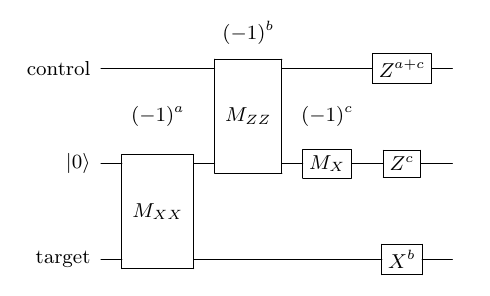
\includegraphics[scale=0.5]{img/cnotMeasureCircuit.png}\\
	\caption{A Quantum Circuit to implement a measurement based\\
		Controlled-$X_{|\psi\rangle_{control}\rightarrow |\psi\rangle_{target}}$ Gate,
		where $|0\rangle$ is the +1 eigenstate in $\sigma_{z}$-basis.}
	\label{fig:circuit1}
	\end{center}
\end{figure}
\newpage

As can be seen explicitly calculated in the familiar Schroedinger 
picture in Appendix~\ref{sec:calc1}, the circuit from figure~\ref{fig:circuit1}
implements a CNOT-gate from the control qubit to the target qubit.

We will now analyze this circuit in the Heisenberg picture,
finding that it results in an equal output.

\subsubsection{Heisenberg Picture}
In this picture, we focus on the time evolution of operators instead
of states:
\begin{equation}
	A = A(t)
\end{equation}
By considering specifically the operators to which the input state
space is part of those operators eigenstatespace, we can compute
the output of any circuit:
\begin{equation}
	Circuit(|\phi\rangle) = Circuit(A)|\phi\rangle
\end{equation}
if $|\phi\rangle$ is an eigenstate of A.\\
This is true because for any unitary operation on a multi-qubit
System applying A to a circuit implementing operator B:
\begin{align}
	|\psi\rangle \rightarrow^{B} B|\psi\rangle \\
	\Rightarrow^A A|\psi\rangle \rightarrow^{B} AB|\psi\rangle =
	(ABA^{\dagger})A |\psi\rangle
\end{align}
If $A|\psi\rangle = |\psi\rangle$, this simplifies to:
\begin{equation}
	|\psi\rangle \rightarrow (ABA^{\dagger})|\psi\rangle
\end{equation}

Therefore the circuit operator $B\rightarrow (ABA^{\dagger})$. 

We call an operator/gate A, to which the input state is an 
eigenvector, a ``Stabilizer'' of that input state. \\
The ``Stabilizer group'' is a generating subset of the set
of such operators.\\
One notable group of operators is the pauli group. It has the
feature that it is ``complete'', in the sense that any
transformation of a single qubit states into another can be
achieved by sequential application of these transformations.\\
Also, for each $A\in P_{G}, n\in \mathbb{N}: A^{2n}=\mathbb{I}$. 
\\
We therefore use the Pauli Group as generating set for our
stabilizers,
so e.g.\ the input state in figure~\ref{fig:circuit1} is only 
stabilized by $\mathbb{I} \otimes Z \otimes \mathbb{I}$ 
(and trivially $\mathbb{I} \otimes \mathbb{I} \otimes \mathbb{I}$).\\
%In general, given a Measurement M and a density matrix $\rho$, after the Measurement
%$\rho\rightarrow\rho'$ with:
%\begin{equation}
%	\rho'=\frac{M\rho M^{\dag}}{tr(M\rho M^{\dag})}
%\end{equation}
In our case, for the first Measurement in circuit \ref{fig:circuit1}
, A is $\mathbb{I}\otimes Z\otimes\mathbb{I}$ and B is
$\mathbb{I}\otimes\mathbb{I}\otimes\mathbb{I}\pm
	\mathbb{I}\otimes X \otimes X$, so depending on wether
the measurement result is $\pm1$ after the first Measurement,
to obtain the evolved Operator we need to compute:
\begin{equation}
	(\mathbb{I}\otimes Z\otimes\mathbb{I})
	(\mathbb{I}\otimes\mathbb{I}\otimes\mathbb{I}\pm
	\mathbb{I}\otimes X \otimes X) 
	(\mathbb{I}\otimes Z\otimes\mathbb{I})^{\dag}
\end{equation}
This notation quickly becomes quite convoluted, so in the 
following we shall denote the Stabilizer as S, and the 
measurements as $M_{1}^{\pm},M_{2}^{\pm},M_{3}^{\pm}$, where
$M_{1}^{\pm}=\mathbb{I}\otimes\mathbb{I}\otimes\mathbb{I}\pm
\mathbb{I}\otimes X \otimes X$,\\ 
$M_{2}^{\pm}=\mathbb{I}\otimes\mathbb{I}\otimes\mathbb{I}\pm
Z \otimes Z \otimes \mathbb{I}$ and \\
$M_{3}^{\pm}=\mathbb{I}\otimes\mathbb{I}\otimes\mathbb{I}\pm
\mathbb{I} \otimes X \otimes \mathbb{I}$. \\
After the second measurement the system operator evolves to:

\begin{equation}
	M_{2}^{\dagger\pm}M_{2}^{\pm}SM_{1}^{\pm}
\end{equation}

After the third it evolves to:

\begin{equation}
	M_{3}^{\dagger\pm}M_{3}^{\pm}M_{2}^{\dagger\pm}M_{2}^{\pm}SM_{1}^{\pm}
\end{equation}
KP THIS NEEDS CLIFFORD STUFF










